\documentclass{standalone}
\usepackage{tikz}
\usetikzlibrary{patterns, positioning}


\begin{document}
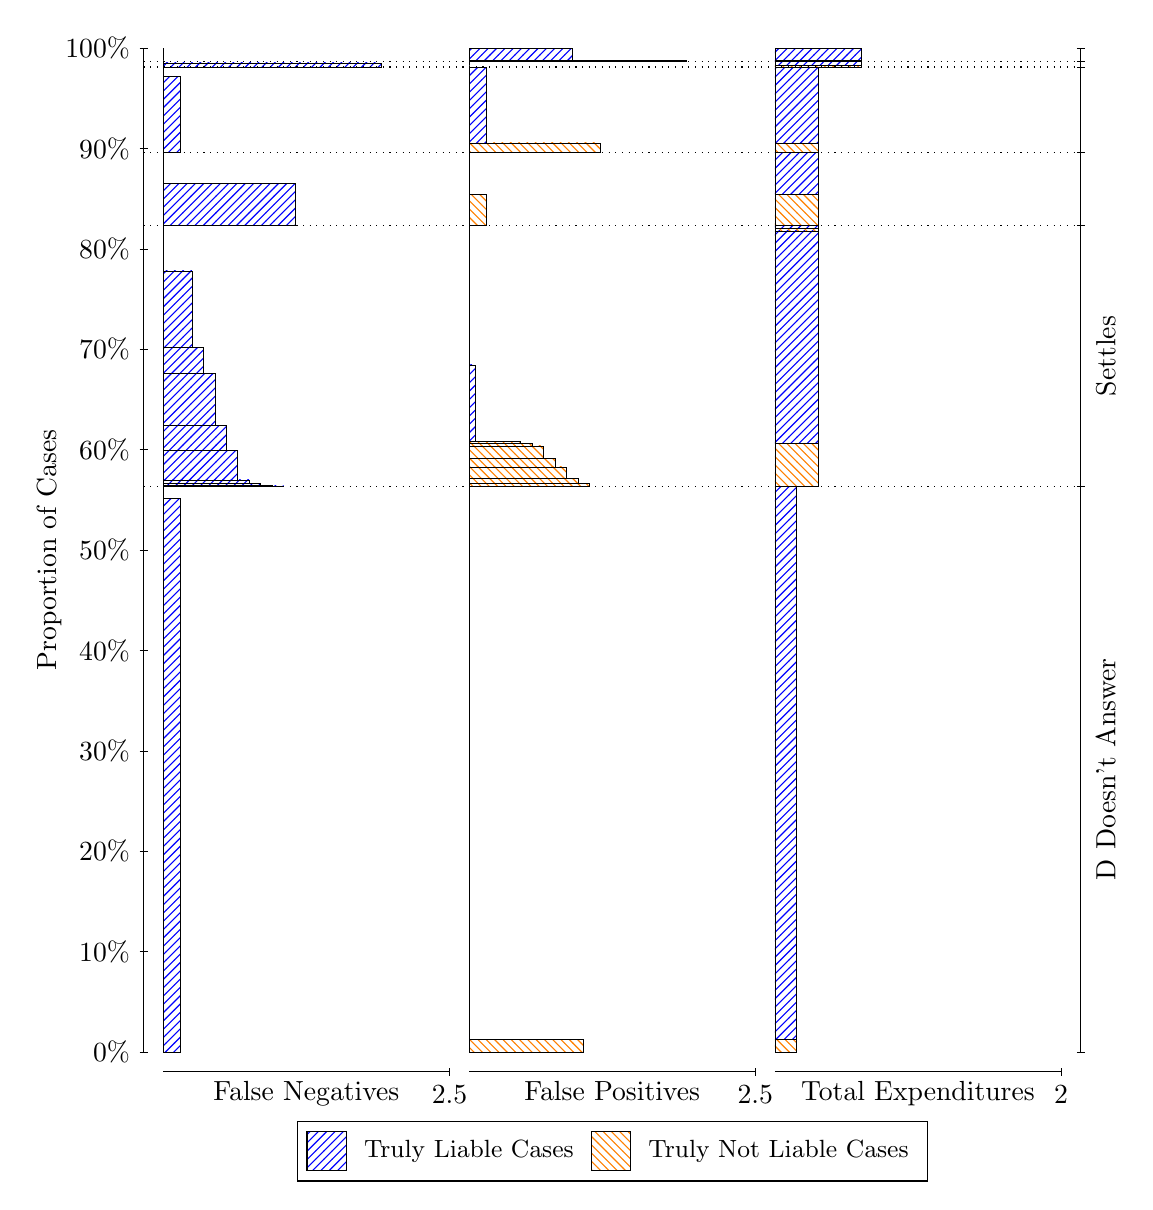
\begin{tikzpicture}
\draw[black, very thin] (1.5,1.75) -- (1.5,14.5);
\node[rotate=90, text=black, anchor=center] at (0.3, 8.125) {Proportion of Cases};
\draw[black, very thin] (1.45,1.75) -- (1.55,1.75);
\node[text=black, anchor=east] at (1.45, 1.75) {0\%};
\draw[black, very thin] (1.45,3.025) -- (1.55,3.025);
\node[text=black, anchor=east] at (1.45, 3.025) {10\%};
\draw[black, very thin] (1.45,4.3) -- (1.55,4.3);
\node[text=black, anchor=east] at (1.45, 4.3) {20\%};
\draw[black, very thin] (1.45,5.575) -- (1.55,5.575);
\node[text=black, anchor=east] at (1.45, 5.575) {30\%};
\draw[black, very thin] (1.45,6.85) -- (1.55,6.85);
\node[text=black, anchor=east] at (1.45, 6.85) {40\%};
\draw[black, very thin] (1.45,8.125) -- (1.55,8.125);
\node[text=black, anchor=east] at (1.45, 8.125) {50\%};
\draw[black, very thin] (1.45,9.4) -- (1.55,9.4);
\node[text=black, anchor=east] at (1.45, 9.4) {60\%};
\draw[black, very thin] (1.45,10.675) -- (1.55,10.675);
\node[text=black, anchor=east] at (1.45, 10.675) {70\%};
\draw[black, very thin] (1.45,11.95) -- (1.55,11.95);
\node[text=black, anchor=east] at (1.45, 11.95) {80\%};
\draw[black, very thin] (1.45,13.225) -- (1.55,13.225);
\node[text=black, anchor=east] at (1.45, 13.225) {90\%};
\draw[black, very thin] (1.45,14.5) -- (1.55,14.5);
\node[text=black, anchor=east] at (1.45, 14.5) {100\%};

\draw[black, very thin] (13.4,1.75) -- (13.4,14.5);
\draw[black, very thin] (13.35,1.75) -- (13.45,1.75);
\node[anchor=west] at (13.35, 1.75) {};
\draw[black, very thin] (13.35,8.9346) -- (13.45,8.9346);
\node[anchor=west] at (13.35, 8.9346) {};
\draw[black, very thin] (13.35,12.243) -- (13.45,12.243);
\node[anchor=west] at (13.35, 12.243) {};
\draw[black, very thin] (13.35,13.177) -- (13.45,13.177);
\node[anchor=west] at (13.35, 13.177) {};
\draw[black, very thin] (13.35,14.259) -- (13.45,14.259);
\node[anchor=west] at (13.35, 14.259) {};
\draw[black, very thin] (13.35,14.334) -- (13.45,14.334);
\node[anchor=west] at (13.35, 14.334) {};
\draw[black, very thin] (13.35,14.5) -- (13.45,14.5);
\node[anchor=west] at (13.35, 14.5) {};

\draw[black, very thin, pattern color=blue, pattern=north east lines] (1.75,1.75) rectangle (1.968,8.7778);
\draw[black, very thin, pattern color=orange, pattern=north west lines] (1.75,8.7778) rectangle (1.75,8.9346);
\draw[black, very thin, pattern color=blue, pattern=north east lines] (1.75,8.9346) rectangle (3.276,8.9387);
\draw[black, very thin, pattern color=blue, pattern=north east lines] (1.75,8.9387) rectangle (3.1307,8.942);
\draw[black, very thin, pattern color=blue, pattern=north east lines] (1.75,8.942) rectangle (2.9853,8.9676);
\draw[black, very thin, pattern color=blue, pattern=north east lines] (1.75,8.9676) rectangle (2.84,9.0155);
\draw[black, very thin, pattern color=blue, pattern=north east lines] (1.75,9.0155) rectangle (2.6947,9.3895);
\draw[black, very thin, pattern color=blue, pattern=north east lines] (1.75,9.3895) rectangle (2.5493,9.7046);
\draw[black, very thin, pattern color=blue, pattern=north east lines] (1.75,9.7046) rectangle (2.404,10.371);
\draw[black, very thin, pattern color=blue, pattern=north east lines] (1.75,10.371) rectangle (2.2587,10.702);
\draw[black, very thin, pattern color=blue, pattern=north east lines] (1.75,10.702) rectangle (2.1133,11.67);
\draw[black, very thin, pattern color=orange, pattern=north west lines] (1.75,11.67) rectangle (1.75,12.243);
\draw[black, very thin, pattern color=blue, pattern=north east lines] (1.75,12.243) rectangle (3.4213,12.777);
\draw[black, very thin, pattern color=orange, pattern=north west lines] (1.75,12.777) rectangle (1.75,13.177);
\draw[black, very thin, pattern color=blue, pattern=north east lines] (1.75,13.177) rectangle (1.968,14.143);
\draw[black, very thin, pattern color=orange, pattern=north west lines] (1.75,14.143) rectangle (1.75,14.259);
\draw[black, very thin, pattern color=blue, pattern=north east lines] (1.75,14.259) rectangle (4.5113,14.312);
\draw[black, very thin, pattern color=orange, pattern=north west lines] (1.75,14.312) rectangle (1.75,14.334);
\draw[black, very thin, pattern color=orange, pattern=north west lines] (1.75,14.334) rectangle (1.75,14.34);
\draw[black, very thin, pattern color=blue, pattern=north east lines] (1.75,14.34) rectangle (1.75,14.5);
\draw[black, very thin, pattern color=orange, pattern=north west lines] (5.6333,1.75) rectangle (7.0867,1.9068);
\draw[black, very thin, pattern color=blue, pattern=north east lines] (5.6333,1.9068) rectangle (5.6333,8.9346);
\draw[black, very thin, pattern color=orange, pattern=north west lines] (5.6333,8.9346) rectangle (7.1593,8.9714);
\draw[black, very thin, pattern color=orange, pattern=north west lines] (5.6333,8.9714) rectangle (7.014,9.0306);
\draw[black, very thin, pattern color=orange, pattern=north west lines] (5.6333,9.0306) rectangle (6.8687,9.1813);
\draw[black, very thin, pattern color=orange, pattern=north west lines] (5.6333,9.1813) rectangle (6.7233,9.2859);
\draw[black, very thin, pattern color=orange, pattern=north west lines] (5.6333,9.2859) rectangle (6.578,9.4482);
\draw[black, very thin, pattern color=orange, pattern=north west lines] (5.6333,9.4482) rectangle (6.4327,9.4794);
\draw[black, very thin, pattern color=orange, pattern=north west lines] (5.6333,9.4794) rectangle (6.4327,9.4814);
\draw[black, very thin, pattern color=orange, pattern=north west lines] (5.6333,9.4814) rectangle (6.2873,9.5043);
\draw[black, very thin, pattern color=orange, pattern=north west lines] (5.6333,9.5043) rectangle (6.142,9.5059);
\draw[black, very thin, pattern color=orange, pattern=north west lines] (5.6333,9.5059) rectangle (5.9967,9.5081);
\draw[black, very thin, pattern color=blue, pattern=north east lines] (5.6333,9.5081) rectangle (5.706,10.476);
\draw[black, very thin, pattern color=blue, pattern=north east lines] (5.6333,10.476) rectangle (5.6333,12.243);
\draw[black, very thin, pattern color=orange, pattern=north west lines] (5.6333,12.243) rectangle (5.8513,12.643);
\draw[black, very thin, pattern color=blue, pattern=north east lines] (5.6333,12.643) rectangle (5.6333,13.177);
\draw[black, very thin, pattern color=orange, pattern=north west lines] (5.6333,13.177) rectangle (7.3047,13.294);
\draw[black, very thin, pattern color=blue, pattern=north east lines] (5.6333,13.294) rectangle (5.8513,14.259);
\draw[black, very thin, pattern color=orange, pattern=north west lines] (5.6333,14.259) rectangle (5.6333,14.281);
\draw[black, very thin, pattern color=blue, pattern=north east lines] (5.6333,14.281) rectangle (5.6333,14.334);
\draw[black, very thin, pattern color=orange, pattern=north west lines] (5.6333,14.334) rectangle (8.3947,14.34);
\draw[black, very thin, pattern color=blue, pattern=north east lines] (5.6333,14.34) rectangle (6.9413,14.5);
\draw[black, very thin, pattern color=orange, pattern=north west lines] (9.5167,1.75) rectangle (9.7892,1.9068);
\draw[black, very thin, pattern color=blue, pattern=north east lines] (9.5167,1.9068) rectangle (9.7892,8.9346);
\draw[black, very thin, pattern color=orange, pattern=north west lines] (9.5167,8.9346) rectangle (10.062,9.4794);
\draw[black, very thin, pattern color=blue, pattern=north east lines] (9.5167,9.4794) rectangle (10.062,12.173);
\draw[black, very thin, pattern color=orange, pattern=north west lines] (9.5167,12.173) rectangle (10.062,12.175);
\draw[black, very thin, pattern color=blue, pattern=north east lines] (9.5167,12.175) rectangle (10.062,12.179);
\draw[black, very thin, pattern color=orange, pattern=north west lines] (9.5167,12.179) rectangle (10.062,12.206);
\draw[black, very thin, pattern color=blue, pattern=north east lines] (9.5167,12.206) rectangle (10.062,12.243);
\draw[black, very thin, pattern color=orange, pattern=north west lines] (9.5167,12.243) rectangle (10.062,12.643);
\draw[black, very thin, pattern color=blue, pattern=north east lines] (9.5167,12.643) rectangle (10.062,13.177);
\draw[black, very thin, pattern color=orange, pattern=north west lines] (9.5167,13.177) rectangle (10.062,13.294);
\draw[black, very thin, pattern color=blue, pattern=north east lines] (9.5167,13.294) rectangle (10.062,14.259);
\draw[black, very thin, pattern color=orange, pattern=north west lines] (9.5167,14.259) rectangle (10.607,14.281);
\draw[black, very thin, pattern color=blue, pattern=north east lines] (9.5167,14.281) rectangle (10.607,14.334);
\draw[black, very thin, pattern color=orange, pattern=north west lines] (9.5167,14.334) rectangle (10.607,14.34);
\draw[black, very thin, pattern color=blue, pattern=north east lines] (9.5167,14.34) rectangle (10.607,14.5);
\draw[black, dotted] (1.5,8.9346) -- (13.4,8.9346);
\draw[black, dotted] (1.5,12.243) -- (13.4,12.243);
\draw[black, dotted] (1.5,13.177) -- (13.4,13.177);
\draw[black, dotted] (1.5,14.259) -- (13.4,14.259);
\draw[black, dotted] (1.5,14.334) -- (13.4,14.334);
\draw[black, very thin] (1.75,1.5) -- (5.3833,1.5);
\node[text=black, anchor=north] at (3.5667, 1.5) {False Negatives};
\draw[black, very thin] (5.3833,1.45) -- (5.3833,1.55);
\node[text=black, anchor=north] at (5.3833, 1.45) {2.5};

\draw[black, very thin] (5.6333,1.5) -- (9.2667,1.5);
\node[text=black, anchor=north] at (7.45, 1.5) {False Positives};
\draw[black, very thin] (9.2667,1.45) -- (9.2667,1.55);
\node[text=black, anchor=north] at (9.2667, 1.45) {2.5};

\draw[black, very thin] (9.5167,1.5) -- (13.15,1.5);
\node[text=black, anchor=north] at (11.333, 1.5) {Total Expenditures};
\draw[black, very thin] (13.15,1.45) -- (13.15,1.55);
\node[text=black, anchor=north] at (13.15, 1.45) {2};

\node[text=black, centered, rotate=90] at (13.72, 5.3423) {D Doesn't Answer};
\node[text=black, centered, rotate=90] at (13.72, 10.589) {Settles};





\draw (7.449999999999999,1.5) node[draw=none] (baseCoordinate) {};
\begin{scope}[align=center]
        \matrix[scale=0.5, draw=black, below=0.5cm of baseCoordinate, nodes={draw}, column sep=0.1cm]{
            \node[rectangle, draw, minimum width=0.5cm, minimum height=0.5cm, pattern color=blue, pattern=north east lines] {}; &
            \node[draw=none, font=\small, text=black] (B) {Truly Liable Cases}; &
            \node[rectangle, draw, minimum width=0.5cm, minimum height=0.5cm, pattern color=orange, pattern=north west lines] {}; &
            \node[draw=none, font=\small, text=black] (B) {Truly Not Liable Cases}; \\
            };
\end{scope}

\end{tikzpicture}
\end{document}